%%%%%%%%%%%%%%%%%%%%%%%%%%%%%%%%%%%%%%%%%%%%%%%%%%%%%%%%%%%%%%%%%%%%%%%%%%%%%%%%%%%%%%%%%
% Khóa luận tốt nghiệp/Tiểu luận 
% LaTeX Template
% Phiên bản 1.0 (tạo ra ngày 05/10/2022)
%
% Template này có thể được download tại:
% https://github.com/cpc1996/HUS-Dissertation-Template
%
% Phiên bản 1.0 được chỉnh sửa bởi:
% Công Phương Cao (congphuongcao@gmail.com)
% Nguyễn Cảnh Việt (vietncp@gmail.com)
%
% Template được tham khảo từ một phiên bản template của:
% Steve Gunn (http://users.ecs.soton.ac.uk/srg/softwaretools/document/templates/)
% Sunil Patel (http://www.sunilpatel.co.uk/thesis-template/)
%
%%%%%%%%%%%%%%%%%%%%%%%%%%%%%%%%%%%%%%%%%%%%%%%%%%%%%%%%%%%%%%%%%%%%%%%%%%%%%%%%%%%%%%%%%


%----------------------------------------------------------------------------------------
%	(KHÔNG CHỈNH SỬA PHẦN NÀY)
%
%	PHẦN 1: CÁC PACKAGE CƠ BẢN VÀ CÁC TÙY CHỈNH VĂN BẢN
%----------------------------------------------------------------------------------------

\documentclass[
12pt,
oneside,
english,
doublespacing,
nolistspacing,
liststotoc,
parskip,
headsepline,
chapterinoneline,
]{HUSdissertation}

% \usepackage[utf8]{inputenc} 
\usepackage[utf8]{vietnam} 
%\usepackage[T1]{fontenc}

\usepackage{mathptmx}
\usepackage{amsmath}
\allowdisplaybreaks

%https://www.overleaf.com/learn/latex/Biblatex_citation_styles
%\usepackage[backend=bibtex,style=authoryear,natbib=true]{biblatex}
\usepackage[backend=bibtex,style=numeric,citestyle=ieee,natbib=true]{biblatex}

\addbibresource{main.bib}

\usepackage[autostyle=true]{csquotes}


%----------------------------------------------------------------------------------------
%	PHẦN 2: CÁC PACKAGE BỔ TRỢ THÊM VÀO TRONG QUÁ TRÌNH BIÊN SOẠN
%----------------------------------------------------------------------------------------

\RequirePackage{setlst}		% Liệt kê/trích dẫn code

\usepackage{multirow}
\usepackage{subfigure}
\usepackage[fontsize=13pt]{scrextend}

%https://www.sascha-frank.com/latex-font-size.html
%https://tex.stackexchange.com/questions/103286/how-to-change-section-subsection-font-size
\usepackage{titlesec}

\titleformat{\section}
{\normalfont\fontsize{13}{13}\bfseries}{\thesection}{1em}{}

\titleformat{\subsection}
{\normalfont\fontsize{13}{13}\bfseries\itshape}{\thesubsection}{1em}{}

%https://tex.stackexchange.com/questions/351961/how-to-indent-code-in-beginverbatim
\usepackage{fancyvrb} 		% Fancy Verbatim
\fvset{tabsize=4,vspace=0pt,fontsize=\footnotesize}

\usepackage{longtable} 		% Bảng dài - Long table

\usepackage[figuresright]{rotating} % Bảng ngang - Sideways table
\usepackage{tabularx}

\usepackage{fontawesome5} 	% Các biểu tượng, ký hiệu đặc biệt

\usepackage{tikz} 			% Vẽ hình
\usetikzlibrary{calc}

\usepackage{indentfirst}	% Lùi đầu dòng ở đầu đoạn văn
\setlength{\parindent}{0.5cm}

%----------------------------------------------------------------------------------------
%	PHẦN 3: THÔNG TIN VỀ Khóa luận tốt nghiệp/Tiểu luận (THESIS INFORMATION)
%----------------------------------------------------------------------------------------

\author{Nhóm 2} 			% Ví dụ: "Nguyễn Thị Thu Thảo"
\thesistitle{\normalsize{Ứng dụng lập trình song song CUDA C++ trong xử lý và phân tích khối dữ liệu ảnh y khoa 3D}} % Tên đồ án

\supervisor {TS. Nguyễn Hoàng Trung} 	% Ví dụ: "PGS. TS. Nguyễn Ngọc Long"
\supervisorr{} 	% Tên này nếu không có thì để trống!

\field{Kỹ thuật điện tử và tin học} 					% Ví dụ: "Ngành Vật lý", "Ngành Hóa học", v.v.
\program{Chương trình đào tạo chuẩn} 			% Ví dụ: "Chương trình đào tạo chuẩn", "Chương trình đào tạo cử nhân tài năng", v.v.
\doctype{Đề tài môn Lập Trình Song Song} % Điền vào đây: "Khóa luận tốt nghiệp đại học hệ chính quy" hoặc "Tiểu luận"

\university{\href{http://hus.vnu.edu.vn}{Trường Đại học Khoa học Tự nhiên}}
\department{\href{http://hus.vnu.edu.vn/gioi-thieu/co-cau-to-chuc/khoa-truc-thuoc/khoa-vat-ly.html}{Khoa Vật lý}}

\AtBeginDocument{
	\hypersetup{pdftitle=\ttitle}
	\hypersetup{pdfauthor=\authorname}
}
\begin{document}

\lstset{style=codeC}	% Thiết lập ngôn ngữ C++ là ngôn ngữ mặc định cho phần liệt kê source code của cả bài

\frontmatter 			% Sử dụng hệ thống đánh số La Mã (i, ii, iii, iv...) cho những trang trước phần mục lục

\pagestyle{plain} 


%----------------------------------------------------------------------------------------
%	(KHÔNG CHỈNH SỬA PHẦN NÀY)
%
%	PHẦN 4: TRANG TIÊU ĐỀ/TRANG BÌA (TITLE PAGE)
%----------------------------------------------------------------------------------------

% TRANG BÌA CHÍNH:
\include{main-cover}

% TRANG BÌA PHỤ:
\include{sub-cover}


%----------------------------------------------------------------------------------------
%	PHẦN 5: DANH NGÔN (QUOTES)
%----------------------------------------------------------------------------------------

% \vspace*{0.2\textheight}

% \noindent\enquote{\itshape 
% 	Cái tôi và sự hiểu biết tỷ lệ nghịch với nhau. Hiểu biết càng nhiều cái tôi càng bé. Hiểu biết càng ít, cái tôi càng to.
% }\bigbreak

% \hfill Albert Einstein


%----------------------------------------------------------------------------------------
%	PHẦN 6: LỜI CẢM ƠN (ACKNOWLEDGEMENTS)
%----------------------------------------------------------------------------------------

\begin{acknowledgements}
	\addchaptertocentry{\acknowledgementname}
	\thispagestyle{empty}
	
	Trước hết, chúng em xin bày tỏ lòng biết ơn chân thành và sâu sắc đến TS. Nguyễn Hoàng Trung người đã tận tình hướng dẫn, hỗ trợ và đồng hành cùng chúng em trong suốt quá trình học tập cũng như thực hiện báo cáo môn Lập trình song song.

	Đề tài ``Ứng dụng lập trình song song CUDA C++ trong xử lý và phân tích khối dữ liệu ảnh y khoa 3D'' là cơ hội quý báu để chúng em có thể vận dụng những kiến thức đã học vào thực tế, đồng thời tiếp cận sâu hơn với lĩnh vực tính toán song song và xử lý ảnh y tế. Trong suốt quá trình thực hiện đề tài, chúng em đã nhận được rất nhiều sự chỉ bảo tận tình, những góp ý chuyên môn quý báu và sự động viên từ thầy. Đây không chỉ là nguồn hỗ trợ quan trọng giúp chúng em hoàn thành đề tài mà còn là nền tảng giúp chúng em nâng cao tư duy nghiên cứu và kỹ năng làm việc thực tế.

	Thông qua báo cáo này, chúng em cũng nhận thức rõ rằng kiến thức và kinh nghiệm của bản thân vẫn còn nhiều hạn chế, vì vậy bài làm khó tránh khỏi những thiếu sót. Chúng em rất mong nhận được những ý kiến đóng góp và nhận xét từ thầy để có thể tiếp tục hoàn thiện bản thân cũng như nâng cao chất lượng nghiên cứu trong tương lai.

	Cuối cùng, chúng em xin kính chúc thầy luôn mạnh khỏe, hạnh phúc và gặt hái nhiều thành công trong công tác giảng dạy cũng như nghiên cứu khoa học.

\end{acknowledgements}


%----------------------------------------------------------------------------------------
%	(KHÔNG CHỈNH SỬA PHẦN NÀY)
%
%	PHẦN 7: MỤC LỤC (LIST OF CONTENTS/FIGURES/TABLES PAGES)
%----------------------------------------------------------------------------------------

\begin{spacing}{1.15}
	\tableofcontents 	% In ra mục lục chính
\end{spacing}

\begin{spacing}{1.15}
	\listoffigures 		% In ra danh sách hình vẽ
\end{spacing}

\begin{spacing}{1.15}
	\listoftables		% In ra danh sách bảng
\end{spacing}


%----------------------------------------------------------------------------------------
%	PHẦN 8: DANH SÁCH TÊN VIẾT TẮT (ABBREVIATIONS)
%----------------------------------------------------------------------------------------

\begin{abbreviations}{ll} % Thêm danh sách tên viết tắt (dưới dạng một bảng có 2 cột)
\textbf{CUDA} & \textbf{C}ompute \textbf{U}nified \textbf{D}evice \textbf{A}rchitecture \\
\textbf{GPU} & \textbf{G}raphics \textbf{P}rocessing \textbf{U}nit \\
\textbf{CPU} & \textbf{C}entral \textbf{P}rocessing \textbf{U}nit \\
\textbf{VRAM} & \textbf{V}ideo \textbf{R}andom \textbf{A}ccess \textbf{M}emory \\
\textbf{RAM} & \textbf{R}andom \textbf{A}ccess \textbf{M}emory \\
\textbf{MIP} & \textbf{M}aximum \textbf{I}ntensity \textbf{P}rojection \\
\textbf{GLCM} & \textbf{G}ray-\textbf{L}evel \textbf{C}o-occurrence \textbf{M}atrix \\
\textbf{OCT} & \textbf{O}ptical \textbf{C}oherence \textbf{T}omography \\
\textbf{OCTA} & \textbf{O}ptical \textbf{C}oherence \textbf{T}omography \textbf{A}ngiography \\
\textbf{CT} & \textbf{C}omputed \textbf{T}omography \\
\textbf{MRI} & \textbf{M}agnetic \textbf{R}esonance \textbf{I}maging \\
\textbf{PET} & \textbf{P}ositron \textbf{E}mission \textbf{T}omography \\
\textbf{CAD} & \textbf{C}omputer-\textbf{A}ided \textbf{D}iagnosis \\
\textbf{3D} & \textbf{3}-\textbf{D}imensional \\
\textbf{2D} & \textbf{2}-\textbf{D}imensional \\
\textbf{I/O} & \textbf{I}nput/\textbf{O}utput \\
\end{abbreviations}


%----------------------------------------------------------------------------------------
%	PHẦN 9: CÁC HẰNG SỐ VẬT LÝ/THÔNG SỐ KĨ THUẬT (PHYSICAL CONSTANTS/OTHER DEFINITIONS)
%----------------------------------------------------------------------------------------

% \begin{constants}{lr@{${}={}$}l} % Thêm danh sách các hằng số (dưới dạng một bảng có 3 cột)

% %	Lệnh \SI{}{} được cung cấp bởi gói siunitx, hãy đọc tài liệu hướng dẫn để biết cách sử dụng nó

% %	Tên hằng số 	 & $Biểu tượng$	& $Hằng số$ cùng với đơn vị\\
% 	Vận tốc ánh sáng & $c_{0}$		& \SI{2.99792458e8}{\meter\per\second} (chính xác)\\

% \end{constants}


%----------------------------------------------------------------------------------------
%	PHẦN 10: DANH SÁCH KÝ HIỆU (SYMBOLS)
%----------------------------------------------------------------------------------------

% \begin{symbols}{lll} % Thêm danh sách các ký hiệu (dưới dạng một bảng có 3 cột)

% %   Ký hiệu	& Ý nghĩa		& Đơn vị \\
% 	$a$		& khoảng cách	& \si{\meter} \\
% 	$P$		& công suất		& \si{\watt} (\si{\joule\per\second}) \\

% 	\addlinespace % Khoảng cách để phân biệt giữa ký hiệu Latin với ký hiệu La Mã

% 	$\omega$ & tần số góc	& \si{\radian} \\

% \end{symbols}


%----------------------------------------------------------------------------------------
%	(KHÔNG CHỈNH SỬA PHẦN NÀY)
%
%	PHẦN 11: LỜI ĐỀ TẶNG (DEDICATION)
%----------------------------------------------------------------------------------------

%\dedicatory{Dành tặng/Dành cho/Gửi tới\ldots} 


%----------------------------------------------------------------------------------------
%	PHẦN 12: NỘI DUNG/CÁC CHƯƠNG Khóa luận tốt nghiệp/Tiểu luận (THESIS CONTENT - CHAPTERS)
%----------------------------------------------------------------------------------------

\mainmatter % Bắt đầu đánh số trang (1,2,3...)

\pagestyle{plain}

% Hãy thêm những chương (chapter) của khóa luận/tiểu luận vào thư mục Chapters
% Hãy bỏ chú thích những dòng nếu bạn đã bổ sung những chương vào

\include{Chapters/Chapter0}
% Chương 1

\chapter{TỔNG QUAN ĐỀ TÀI}

\label{Chapter1}

%----------------------------------------------------------------------------------------

\newcommand{\keyword}[1]{\textbf{#1}}
\newcommand{\tabhead}[1]{\textbf{#1}}
\newcommand{\code}[1]{\texttt{#1}}
\newcommand{\file}[1]{\texttt{\bfseries#1}}
\newcommand{\option}[1]{\texttt{\itshape#1}}

%----------------------------------------------------------------------------------------

\section{Mở đầu}

Trong bức tranh tổng thể của nền y học hiện đại, chẩn đoán hình ảnh kỹ thuật số định hình như một công cụ then chốt, quyết định tính chính xác của quy trình phát hiện bệnh lý, theo dõi tiến triển lâm sàng và xây dựng phác đồ điều trị. Sự tiến bộ mang tính bước ngoặt của các công nghệ hình ảnh tiên tiến như chụp cắt lớp vi tính (CT), cộng hưởng từ (MRI), hay chụp cắt lớp phát xạ positron (PET) đã tái định nghĩa khả năng quan sát y khoa. Đặc biệt, sự ra đời của công nghệ chụp cắt lớp quang học và mạch máu quang học (\textit{Optical Coherence Tomography/Angiography} - OCT/OCTA) đã cho phép các chuyên gia y tế tiếp cận cấu trúc vi mạch và mô sinh học dưới dạng không gian ba chiều (3D) ở độ phân giải siêu cao. Khả năng hiển thị trực quan và chi tiết các khối bất thường này đóng vai trò tối quan trọng trong việc nâng cao chất lượng và tính kịp thời cho các quyết định lâm sàng.

Tuy nhiên, việc nâng cao độ phân giải hình ảnh lại đặt ra một thách thức lớn về mặt kỹ thuật do sự bùng nổ của khối lượng dữ liệu thô. Một khối dữ liệu ảnh 3D (Volume dữ liệu) biểu diễn hệ thống vi mạch thường bao phủ một không gian quy mô lớn, chứa từ hàng trăm triệu cho đến hơn một tỷ điểm dữ liệu (\textit{voxel}). Khi đối mặt với khối lượng thông tin đồ sộ này, việc triển khai chuỗi toán tử xử lý từ lọc nhiễu, phân mảnh cấu trúc cho đến trích xuất đặc trưng trên kiến trúc tính toán tuần tự của các bộ vi xử lý trung tâm (CPU) truyền thống lập tức bộc lộ những hạn chế cố hữu. Sự chậm trễ trong thời gian xử lý tạo ra một nút thắt cổ chai hệ thống nghiêm trọng, hoàn toàn không tương thích với yêu cầu chẩn đoán thời gian thực hoặc phản ứng nhanh trong các tình huống y tế khẩn cấp, đồng thời dẫn đến hiệu suất khai thác tài nguyên phần cứng thấp.

Để vượt qua rào cản hiệu năng của kiến trúc cũ, xu hướng dịch chuyển sang mô hình tính toán song song khối lượng lớn thông qua nền tảng công nghệ CUDA của NVIDIA trên các bộ xử lý đồ họa (GPU) được xem là một bước đi đột phá và mang tính tất yếu. Nhờ sở hữu kiến trúc phần cứng tối ưu cho phép điều phối và thực thi đồng thời hàng chục ngàn luồng dữ liệu (\textit{threads}), GPU mở ra khả năng tăng tốc vượt trội cho các tác vụ lặp đi lặp lại trên lưới ma trận đa chiều, từ đó thiết lập một đường ống xử lý dữ liệu (\textit{Data Pipeline}) liền mạch, đồng bộ cho các hệ thống chẩn đoán thông minh.

Hướng tới mục tiêu giải quyết triệt để bài toán hiệu năng tính toán trong phân tích ảnh y khoa, đề tài “Ứng dụng lập trình song song CUDA C++ trong xử lý và phân tích khối dữ liệu ảnh y khoa 3D” đã được nghiên cứu và thực hiện. Trên cơ sở thực nghiệm với khối ảnh mô phỏng từ bộ dữ liệu vi mạch mu bàn tay (\textit{Dorsum Hand OCT/OCTA}), nghiên cứu tập trung xây dựng một hệ thống xử lý tốc độ cao được tự động hóa hoàn toàn thông qua cấu trúc mã nguồn CUDA C++. Tiến trình xử lý của hệ thống bắt đầu bằng khâu giảm chiều không gian thông qua kỹ thuật ép khối dữ liệu ảnh 3D thành bản đồ bề mặt 2D (\textit{En-face/Maximum Intensity Projection}) để cung cấp góc nhìn tổng quan về mạng lưới mạch máu. Tiếp theo, hệ thống áp dụng các bộ lọc không gian cửa sổ trượt (Mean Blur) chạy song song song hành cùng thuật toán phân ngưỡng nhị phân nhằm triệt tiêu nhiễu nền và phân tách chính xác cấu trúc hình học của hệ thống vi mạch. Từ kết quả ảnh đã tiền xử lý, nhánh phân tích hình thái sẽ tự động đo lường mật độ mạng lưới mạch máu (\textit{Vessel Density}) thông qua các toán tử đếm nguyên tử (\textit{Atomic Operations}), trong khi nhánh phân tích kết cấu chịu trách nhiệm khởi tạo ma trận đồng xuất hiện mức xám (GLCM) kích thước $256 \times 256$ ngay trên bộ nhớ GPU để trích xuất các đặc trưng toán học chuyên sâu của mô sinh học bao gồm độ tương phản (Contrast), độ đồng nhất (Homogeneity) và năng lượng (Energy).
%----------------------------------------------------------------------------------------

% Chương 2

\chapter{CƠ SỞ LÝ THUYẾT}

\label{Chapter2}

%----------------------------------------------------------------------------------------

\section{Tổng quan về khối dữ liệu 3D trong Y khoa}

Nếu như trong ảnh 2D, đơn vị cơ bản cấu tạo nên bức ảnh là Điểm ảnh (Pixel -- Picture Element), thì trong không gian 3D, phần tử cơ bản được gọi là \textbf{Điểm thể tích (Voxel -- Volume Element)}. Mỗi voxel trong khối dữ liệu chứa một giá trị cường độ sáng tương ứng với mật độ quang học hoặc cấu trúc vật lý của mô tại tọa độ không gian $(x, y, z)$ đó~\cite{gonzalez2018digital}.

Khối dữ liệu 3D thực chất là một tập hợp của hàng trăm đến hàng ngàn lát cắt 2D (Slices) được xếp chồng lên nhau dọc theo trục $Z$. Do kích thước dữ liệu khổng lồ (thường lên đến hàng tỷ voxel), việc truy xuất và xử lý khối dữ liệu này đòi hỏi tài nguyên bộ nhớ lớn và năng lực tính toán tốc độ cao.

%----------------------------------------------------------------------------------------

\section{Kiến trúc Lập trình song song CUDA}

CUDA (Compute Unified Device Architecture) là một nền tảng tính toán song song và mô hình lập trình do NVIDIA phát triển, cho phép tận dụng tối đa sức mạnh của các Bộ xử lý đồ họa (GPU) để giải quyết các bài toán tính toán phức tạp~\cite{nvidia_cuda_guide}.

\begin{figure}[h]
    \centering
    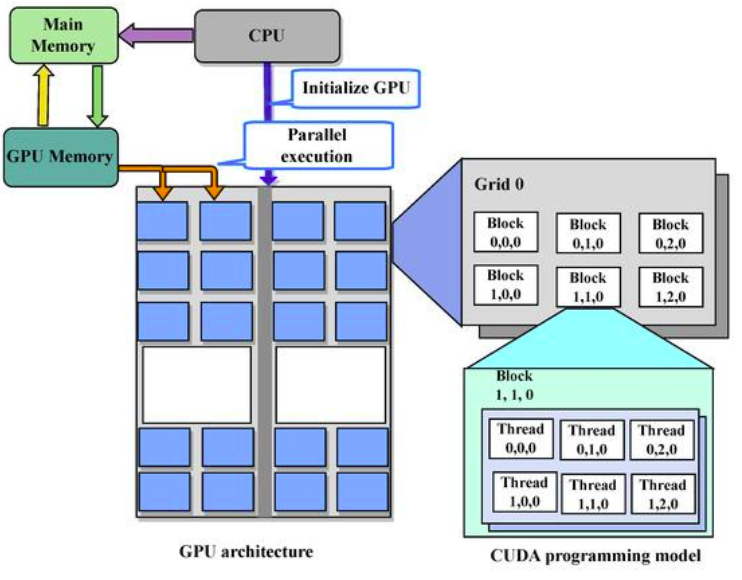
\includegraphics[height=8cm, keepaspectratio]{Figures/Chapter/1.png}
    \caption{Mô hình lập trình CUDA}
    \label{fix:chapter1_1}
\end{figure}

Mô hình lập trình CUDA phân chia hệ thống thành hai phần chính:

\begin{itemize}
    \item \textbf{Host (Máy chủ):} Bao gồm CPU và bộ nhớ chính (RAM), đóng vai trò điều khiển luồng chương trình, cấu hình thông số và khởi tạo dữ liệu.
    \item \textbf{Device (Thiết bị):} Bao gồm GPU và bộ nhớ video (VRAM), chuyên đảm nhận các tác vụ tính toán chuyên sâu mang tính lặp đi lặp lại.
\end{itemize}

\textbf{Cấu trúc phân cấp luồng (Thread Hierarchy):} Để quản lý hàng chục ngàn phép tính diễn ra cùng lúc, CUDA tổ chức các luồng thực thi theo ba cấp độ:

\begin{enumerate}
    \item \textbf{Thread (Luồng):} Đơn vị tính toán nhỏ nhất. Mỗi Thread thường chịu trách nhiệm tính toán cho đúng một điểm ảnh (pixel/voxel).
    \item \textbf{Block (Khối):} Tập hợp của nhiều Thread. Các Thread trong cùng một Block có thể giao tiếp và chia sẻ dữ liệu với nhau thông qua bộ nhớ chung (Shared Memory).
    \item \textbf{Grid (Lưới):} Tập hợp của nhiều Block. Kích thước của Grid được thiết kế để bao phủ toàn bộ không gian của khối dữ liệu cần xử lý.
\end{enumerate}

%----------------------------------------------------------------------------------------

\section{Cơ sở thuật toán nhánh phân tích mạch máu (Vessel Analysis)}

\subsection{Thuật toán chiếu ảnh cường độ tối đa (MIP)}

MIP (Maximum Intensity Projection) là phương pháp nén khối dữ liệu 3D thành bản đồ 2D~\cite{defined_mip}. Thuật toán mô phỏng việc chiếu các tia sáng dọc theo trục $Z$ của khối. Trên mỗi đường truyền của tia từ mặt trên xuống mặt đáy, thuật toán sẽ lấy giá trị voxel có cường độ sáng lớn nhất để chiếu lên mặt phẳng 2D:
\begin{equation}
    I_{MIP}(x,y) = \max_{z=0}^{D-1} V(x, y, z)
    \label{eq:mip}
\end{equation}
trong đó $V(x, y, z)$ là giá trị voxel tại tọa độ $(x, y, z)$ và $D$ là chiều sâu của khối dữ liệu.

\begin{figure}[h]
    \centering
    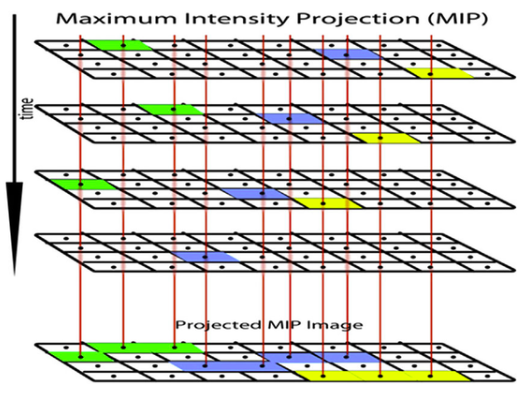
\includegraphics[height=8cm, keepaspectratio]{Figures/Chapter/2.png}
    \caption{Mô hình lập trình CUDA}
    \label{fix:chapter1_2}
\end{figure}

Do mạch máu thường có mức độ phản xạ quang học sáng hơn so với mô nền, thuật toán MIP giúp trích xuất toàn bộ mạng lưới mạch máu ẩn bên trong lớp da lên một bức ảnh bề mặt duy nhất.

\subsection{Bộ lọc trung bình (Mean Filter)}

Trong quá trình thu nhận tín hiệu từ các thiết bị chụp cắt lớp (như CT, MRI hay OCT), hình ảnh thường bị suy giảm chất lượng do sự xuất hiện của các loại nhiễu ngẫu nhiên, đặc biệt là nhiễu hạt (\textit{speckle noise}) và nhiễu Gaussian. Để loại bỏ các thành phần nhiễu này và cải thiện tỷ số tín hiệu trên nhiễu (SNR), một bộ lọc không gian tuyến tính — cụ thể là bộ lọc trung bình (\textit{Mean Blur}) với kích thước cửa sổ (kernel) $3 \times 3$ — được áp dụng lên từng điểm ảnh.

Giá trị của điểm ảnh sau khi làm mịn tại tọa độ $(x, y)$ được xác định bằng trung bình cộng giá trị của chính nó và các điểm ảnh lân cận trong phạm vi cửa sổ lọc, tuân theo công thức toán học sau:

\begin{equation}
I_{\text{blur}}(x, y) = \frac{1}{9} \sum_{i=-1}^{1} \sum_{j=-1}^{1} I(x + i, y + j)
\label{eq:mean_filter}
\end{equation}

Trong đó:
\begin{itemize}
    \item $I(x, y)$ là giá trị cường độ sáng của điểm ảnh gốc tại tọa độ $(x, y)$.
    \item $I_{\text{blur}}(x, y)$ là giá trị cường độ sáng của điểm ảnh sau khi đã áp dụng bộ lọc trung bình.
    \item $i$ và $j$ là các chỉ số dịch chuyển trong không gian hai chiều của cửa sổ lọc kích thước $3 \times 3$.
\end{itemize}

Về mặt hiệu quả xử lý, kỹ thuật lọc không gian này đóng vai trò quan trọng trong việc làm mịn vùng nền mô xung quanh, giảm thiểu các biến động tần số cao do nhiễu gây ra. Đồng thời, quá trình làm mịn cấu trúc này còn hỗ trợ kết nối các phân đoạn mạch máu bị đứt gãy cục bộ do suy hao tín hiệu, tạo điều kiện thuận lợi cho các bước phân đoạn ảnh (\textit{segmentation}) và trích xuất hình thái mạch máu tiếp theo.

\subsection{Thuật toán phân ngưỡng nhị phân (Thresholding)}

Sau giai đoạn làm mịn và giảm nhiễu, thuật toán phân ngưỡng nhị phân (\textit{Binary Thresholding}) được áp dụng như một bước tiền xử lý quyết định nhằm tách biệt đối tượng quan tâm (mạch máu, tổn thương) ra khỏi vùng nền cấu trúc mô. Bản chất của kỹ thuật này là chuyển đổi một ảnh xám (\textit{grayscale image}) có dải giá trị liên tục thành một ảnh nhị phân (\textit{binary image}) chỉ bao gồm hai màu đen và trắng thuần túy.

Quá trình chuyển đổi được thực hiện bằng cách so sánh cường độ sáng của từng điểm ảnh $I(x, y)$ tại vị trí tọa độ $(x, y)$ với một giá trị ngưỡng cường độ cố định $T$ (chọn trước dựa trên thực nghiệm hoặc giải thuật tối ưu, ví dụ: $T = 140$). Hàm toán học phân ngưỡng được định nghĩa như sau:

\begin{equation}
I_{\text{binary}}(x, y) = 
\begin{cases} 
255 & \text{nếu } I(x, y) > T \\ 
0 & \text{nếu } I(x, y) \le T 
\end{cases}
\label{eq:thresholding}
\end{equation}

Trong đó:
\begin{itemize}
    \item $I(x, y)$ là giá trị mức xám gốc của điểm ảnh tại tọa độ $(x, y)$, thường nằm trong đoạn $[0, 255]$ đối với ảnh 8-bit.
    \item $T$ là ngưỡng cường độ quyết định (\textit{threshold value}).
    \item $I_{\text{binary}}(x, y)$ là giá trị của điểm ảnh sau khi nhị phân hóa. Giá trị $255$ đại diện cho các điểm ảnh thuộc vùng trắng (đối tượng mạch máu cần giữ lại), và giá trị $0$ đại diện cho vùng đen (nền ảnh).
\end{itemize}

Kết quả của quá trình phân ngưỡng nhị phân này tạo ra một bản đồ mặt nạ (\textit{binary mask}) rõ ràng và cô đọng. Đây là cơ sở dữ liệu đầu vào cốt lõi và bắt buộc để hệ thống tiến hành tính toán chỉ số Mật độ mạch máu (\textit{Vessel Density - VD}) — một thông số lâm sàng quan trọng bậc nhất trong việc đánh giá tình trạng tưới máu mô và chẩn đoán các bệnh lý vi mạch.


\subsection{Tính toán Mật độ mạch máu (Vessel Density)}

Sau khi hoàn thành quá trình phân ngưỡng nhị phân, toàn bộ cấu trúc hình thái của mạng lưới mạch máu đã được bóc tách hoàn toàn khỏi nền mô dưới dạng các điểm ảnh màu trắng (giá trị $255$). Lúc này, chỉ số Mật độ mạch máu (\textit{Vessel Density - VD}) được tiến hành tính toán. Đây là một đại lượng thông số định lượng quan trọng, phản ánh tỷ lệ diện tích được tưới máu trên một đơn vị diện tích khảo sát.

Về mặt toán học, mật độ mạch máu được xác định bằng tỷ lệ phần trăm giữa tổng số lượng điểm ảnh được định danh là mạch máu trên tổng số lượng điểm ảnh toàn vùng bề mặt ảnh khảo sát. Công thức tính toán được biểu diễn như sau:

\begin{equation}
\text{Vessel Density (\%)} = \frac{N_{\text{vessel}}}{W \times H} \times 100\%
\label{eq:vessel_density}
\end{equation}

Trong đó:
\begin{itemize}
    \item $N_{\text{vessel}}$ là tổng số lượng điểm ảnh thuộc mạng lưới mạch máu (tức là số lượng các điểm ảnh có giá trị bằng $255$ trong ảnh nhị phân đầu ra của bước trước).
    \item $W$ (\textit{Width}) là chiều rộng của vùng ảnh khảo sát, tính theo đơn vị pixel.
    \item $H$ (\textit{Height}) là chiều cao của vùng ảnh khảo sát, tính theo đơn vị pixel.
    \item Tích số $W \times H$ đại diện cho tổng diện tích bề mặt (tổng số lượng điểm ảnh) của toàn bộ vùng phân tích (\textit{Region of Interest - ROI}).
\end{itemize}

Chỉ số \textit{Vessel Density} thu được là một tham số khách quan và có độ tin cậy cao. Trong lâm sàng, sự suy giảm hoặc biến động bất thường của chỉ số phần trăm này là dấu hiệu chỉ thị quan trọng cho các tổn thương thiếu máu cục bộ, teo mạch vi tuần hoàn, hoặc sự tăng sinh mạch máu bất thường trong các bệnh lý ác tính.

%----------------------------------------------------------------------------------------

\section{Phân tích kết cấu mô bằng ma trận GLCM (Texture Analysis)}

Để phân tích sâu hơn các đặc tính vi mô của mô tổn thương — những đặc điểm thường phân bố phức tạp và khó nhận diện bằng mắt thường — phương pháp phân tích kết cấu dựa trên Ma trận đồng xuất hiện mức xám (\textit{Gray-Level Co-Occurrence Matrix - GLCM}) được áp dụng. Đây là một kỹ thuật thống kê không gian bậc hai (\textit{second-order spatial statistics}), cho phép định lượng mối quan hệ cấu trúc giữa các cặp điểm ảnh dựa trên vị trí tương đối của chúng trong không gian hai chiều.

Giả sử vùng ảnh khảo sát có dải giá trị cường độ sáng gồm $L$ mức xám (đối với ảnh số chuẩn 8-bit, mức xám chạy từ $0$ đến $255$, tương ứng với $L = 256$). Khi đó, ma trận GLCM thu được sẽ là một ma trận vuông kích thước $L \times L$ (ví dụ: $256 \times 256$). Một phần tử tại vị trí hàng $i$, cột $j$ (ký hiệu là $C(i, j)$) lưu trữ tần suất xuất hiện của một cặp điểm ảnh: trong đó điểm ảnh thứ nhất có mức xám $i$ và điểm ảnh thứ hai có mức xám $j$, thỏa mãn một mối quan hệ không gian được xác định bởi khoảng cách dịch chuyển $d$ (tính theo pixel) và hướng góc $\theta$ (các hướng thông dụng là $\theta \in \{0^\circ, 45^\circ, 90^\circ, 135^\circ\}$).

Để loại bỏ sự phụ thuộc vào kích thước vùng ảnh phân tích và phục vụ cho việc tính toán các đặc trưng thống kê, ma trận tần suất thô $C(i, j)$ cần được chuẩn hóa thành ma trận xác suất $P(i, j)$ theo công thức:

\begin{equation}
P(i, j) = \frac{C(i, j)}{\sum_{i=0}^{L-1} \sum_{j=0}^{L-1} C(i, j)}
\label{eq:glcm_normalization}
\end{equation}

Từ ma trận xác suất đồng xuất hiện $P(i, j)$, các đặc trưng kết cấu mang thông tin kiểu hình lâm sàng quan trọng được trích xuất cụ thể như sau:

\subsection{Độ tương phản (Contrast)}
Đại lượng này đo lường mức độ biến thiên và sự khác biệt về cường độ sáng cục bộ giữa các cặp điểm ảnh lân cận trong toàn bộ vùng ảnh khảo sát. Công thức tính toán được xác định bởi:

\begin{equation}
\text{Contrast} = \sum_{i=0}^{L-1} \sum_{j=0}^{L-1} |i - j|^2 \cdot P(i, j)
\label{eq:contrast}
\end{equation}

Về mặt ý nghĩa, nếu một vùng mô có độ tương phản cao, điều đó chứng tỏ có sự chênh lệch lớn về mức xám giữa các điểm ảnh đứng cạnh nhau, biểu thị một kết cấu bề mặt thô ráp, có nếp gấp sâu hoặc chứa các cấu trúc thay đổi đột ngột (ví dụ như ranh giới giữa mô lành và khối u). Ngược lại, giá trị này thấp đối với các vùng mô có kết cấu mịn và đồng đều.

\subsection{Độ đồng nhất (Homogeneity)}
Độ đồng nhất (\textit{Homogeneity}), hay còn gọi là Mô-men chênh lệch ngược (\textit{Inverse Difference Moment - IDM}), dùng để đo lường sự chặt chẽ và mức độ tập trung trong phân bố của các phần tử trên ma trận GLCM so với đường chéo chính. Công thức toán học được biểu diễn như sau:

\begin{equation}
\text{Homogeneity} = \sum_{i=0}^{L-1} \sum_{j=0}^{L-1} \frac{P(i, j)}{1 + |i - j|}
\label{eq:homogeneity}
\end{equation}

Hàm trọng số $\frac{1}{1 + |i - j|}$ sẽ đạt giá trị lớn nhất khi khoảng cách $|i - j|$ tiến về $0$ (tức là các phần tử nằm sát hoặc nằm ngay trên đường chéo chính, ứng với các cặp điểm ảnh có mức xám bằng hoặc gần bằng nhau). Chỉ số này tỉ lệ thuận với tính đồng nhất của bề mặt mô; giá trị Homogeneity càng cao chứng tỏ vùng mô khảo sát có sự chuyển đổi mức xám rất mượt mà, tĩnh lặng và ít có sự đột biến cấu trúc.

\subsection{Năng lượng (Energy)}
Năng lượng (\textit{Energy}), hay còn được gọi là Mô-men góc thứ hai (\textit{Angular Second Moment - ASM}), là đại lượng dùng để đo lường sự lặp lại của các cặp mức xám, phản ánh độ đồng đều tổng thể (\textit{Uniformity}) của kết cấu hình thái ảnh. Công thức xác định là:

\begin{equation}
\text{Energy} = \sum_{i=0}^{L-1} \sum_{j=0}^{L-1} \left[ P(i, j) \right]^2
\label{eq:energy}
\end{equation}

Khi một vùng ảnh chứa các cấu trúc hoa văn lặp đi lặp lại một cách tuần hoàn, có tổ chức hoặc phân bố mức xám rất tập trung, ma trận xác suất $P(i, j)$ sẽ xuất hiện một vài ô có giá trị xác suất rất cao vượt trội. Phép bình phương $\left[ P(i, j) \right]^2$ sẽ làm khuếch đại các giá trị cao này, dẫn đến tổng chỉ số Energy lớn. Trong phân tích lâm sàng, chỉ số Energy cao đại diện cho các mô có cấu trúc hình thái ổn định, được tổ chức tốt; trong khi giá trị thấp thường cảnh báo một vùng mô hỗn loạn, vô tổ chức (đặc trưng thường thấy ở các vùng mô tăng sinh ác tính hoặc các tế bào ung thư phát triển vô hướng).

%----------------------------------------------------------------------------------------
 
% Chương 3

\chapter{PHƯƠNG PHÁP VÀ KIẾN TRÚC HỆ THỐNG}

\label{Chapter3}

%----------------------------------------------------------------------------------------

\section{Kiến trúc hệ thống tổng quát (System Pipeline)}

Hệ thống xử lý khối ảnh y khoa 3D được thiết kế theo mô hình luồng dữ liệu (Data Pipeline), phân chia rõ ràng các tác vụ giữa CPU (Host) và GPU (Device) nhằm tận dụng tối đa băng thông bộ nhớ và năng lực tính toán song song. Cấu trúc hệ thống bao gồm 3 giai đoạn chính:

\begin{enumerate}
    \item \textbf{Giai đoạn 1: Tiền xử lý dữ liệu I/O (CPU):} Chuyển đổi định dạng dữ liệu đầu vào từ dạng văn bản phân mảnh sang dạng nhị phân nguyên khối.
    
    \item \textbf{Giai đoạn 2: Trích xuất bản đồ 2D (GPU):} Nạp toàn bộ khối dữ liệu 3D lên VRAM và thực thi thuật toán MIP để ép xuống mặt phẳng 2D.
    
    \item \textbf{Giai đoạn 3: Xử lý song song đa nhánh (GPU \& CPU):} Từ bản đồ 2D gốc, luồng thực thi được chia làm hai nhánh độc lập:
    \begin{itemize}
        \item \textit{Nhánh 1 (Vessel Analysis):} Xử lý hình thái mạch máu (Làm mờ $\rightarrow$ Phân ngưỡng $\rightarrow$ Đếm điểm ảnh).
        \item \textit{Nhánh 2 (Texture Analysis):} Xử lý kết cấu mô (Khởi tạo GLCM bằng GPU $\rightarrow$ Trích xuất đặc trưng toán học bằng CPU).
    \end{itemize}
\end{enumerate}

% TODO: Vẽ một Sơ đồ khối ba giai đoạn trên

%----------------------------------------------------------------------------------------

\section{Tối ưu hóa I/O Dữ liệu (Data I/O Optimization)}

Một trong những nút thắt cổ chai lớn nhất của hệ thống ban đầu là quá trình nạp dữ liệu. Dữ liệu gốc được lưu dưới dạng hàng trăm tệp văn bản tĩnh (\code{.txt}), chứa các giá trị mức xám dưới dạng chuỗi ký tự ASCII. Việc yêu cầu CPU mở từng tệp, đọc chuỗi, giải mã thành số thực (float) và chuẩn hóa màu sắc mất rất nhiều thời gian.

Để giải quyết vấn đề này, một module Tiền xử lý dữ liệu (Preprocessor) được xây dựng trên C++. Module này thực hiện các bước sau:

\begin{itemize}
    \item Quét qua toàn bộ các tệp \code{.txt}.
    \item Nén và xuất toàn bộ dữ liệu ra một tệp nhị phân duy nhất (\code{volume\_3d.raw}).
\end{itemize}

Nhờ định dạng Binary \code{.raw}, máy tính có thể nạp hàng tỷ byte dữ liệu trực tiếp vào bộ nhớ RAM và đẩy lên VRAM của GPU trong thời gian ngắn.

%----------------------------------------------------------------------------------------

\section{Thiết kế và Triển khai các hàm Kernel CUDA}

Để thực thi song song trên GPU, mạng lưới luồng (Grid) được thiết kế dựa trên kích thước của bề mặt ảnh 2D ($W \times H$). Cụ thể, ảnh được chia thành các Block nhỏ kích thước $16 \times 16$ threads. Số lượng Block được tự động tính toán bù trừ để đảm bảo phủ kín toàn bộ diện tích ảnh mà không bị tràn viền.

\subsection{Kernel Chiếu ảnh cường độ tối đa (MIP\_Projection)}

Thuật toán MIP duyệt qua toàn bộ chiều sâu $D$ của khối ảnh. Trong không gian 3D, mỗi luồng (thread) được gắn tọa độ $(x, y)$ tương ứng với một điểm ảnh trên mặt phẳng đích. GPU phân công mỗi luồng chỉ chạy 1 vòng lặp dọc theo trục $Z$. Luồng sẽ duyệt qua các giá trị tại tọa độ $(x, y, z)$ tương ứng, so sánh và lưu trữ giá trị cực đại tìm được vào biến \code{max\_val}, sau đó ghi thẳng vào mảng \code{d\_mip} 2D.

\subsection{Các Kernel thuộc nhánh Vessel Analysis}

\begin{itemize}
    \item \textbf{Kernel Làm mờ (Mean\_Blur):} Mỗi luồng tại tọa độ $(x, y)$ kiểm tra các điều kiện biên để tránh lỗi truy xuất vùng nhớ (Segmentation fault). Nếu an toàn, luồng sẽ tính tổng cường độ của điểm ảnh đó và 8 điểm lân cận, sau đó chia cho 9 để ra giá trị trung bình và ghi vào ảnh \code{d\_blurred}.
    
    \item \textbf{Kernel Phân ngưỡng (Thresholding):} Các luồng hoạt động hoàn toàn độc lập, thực hiện phép toán rẽ nhánh: Nếu giá trị tại $(x,y)$ vượt qua ngưỡng được cài đặt (ví dụ: 140), gán bằng 255; ngược lại gán bằng 0.
    
    \item \textbf{Kernel Đếm mạch máu (Count\_Vessels):} Để tránh việc hàng ngàn luồng ghi đè lên nhau khi cộng dồn tổng số điểm ảnh trắng, lệnh khóa bộ nhớ \code{atomicAdd()} được sử dụng. Mỗi luồng phát hiện điểm mạch máu sẽ an toàn cộng thêm 1 vào biến con trỏ \code{d\_white\_count} lưu trên VRAM.
\end{itemize}

\subsection{Kernel thuộc nhánh Texture Analysis (GLCM)}

Khác với nhánh trên, tính toán kết cấu yêu cầu đếm tần suất xuất hiện của các cặp điểm ảnh lân cận. Tại hàm \code{Compute\_GLCM}, mỗi luồng xử lý một cặp điểm ảnh (\code{pixel\_1}, \code{pixel\_2}) theo độ dời ngang ($dx = 1, dy = 0$).

Ma trận GLCM $256 \times 256$ được trải phẳng thành mảng 1 chiều kích thước 65.536 phần tử. Chỉ số để cập nhật ma trận được tính toán bằng công thức:
\begin{equation}
    \text{index} = \text{pixel\_1} \times 256 + \text{pixel\_2}
    \label{eq:glcm_index}
\end{equation}

Tại chỉ số này, luồng tiếp tục gọi \code{atomicAdd()} để tăng tần suất cặp mức xám lên 1 đơn vị.

%----------------------------------------------------------------------------------------

\section{Quản lý bộ nhớ và Đồng bộ hóa}

\begin{itemize}
    \item \textbf{Cấp phát:} Sử dụng \code{cudaMalloc} để cấp phát vùng nhớ độc lập trên VRAM cho từng giai đoạn (Khối gốc, Ảnh MIP, Ảnh Blur, Ảnh nhị phân và Ma trận GLCM).
    
    \item \textbf{Làm sạch bộ nhớ:} Trước khi khởi chạy các Kernel đếm tổng hoặc GLCM, bộ nhớ VRAM luôn chứa dữ liệu rác. Hàm \code{cudaMemset} được gọi để ép các vùng nhớ này về 0, đảm bảo tính chính xác tuyệt đối cho \code{atomicAdd}.
    
    \item \textbf{Đồng bộ hóa:} Giữa mỗi bước thực thi Kernel, lệnh \code{cudaDeviceSynchronize()} đóng vai trò là rào chắn (Barrier), bắt buộc CPU phải tạm dừng để chờ toàn bộ hàng chục ngàn luồng của GPU hoàn thành xong công việc hiện tại, mới được phép phát lệnh chạy Kernel tiếp theo, tránh tình trạng lấy kết quả sai lệch.
\end{itemize}

%----------------------------------------------------------------------------------------

% Chương 4

\chapter{KẾT QUẢ THỰC NGHIỆM VÀ ĐÁNH GIÁ}

\label{Chapter4}

%----------------------------------------------------------------------------------------

\section{Môi trường và Dữ liệu thực nghiệm}

Quá trình biên dịch mã nguồn và thực nghiệm đo lường hiệu năng được triển khai trên nền tảng điện toán đám mây Google Colaboratory.

\begin{itemize}
    \item \textbf{Phần cứng (Hardware):} Hệ thống sử dụng máy ảo được cấu hình CPU của Google và bộ xử lý đồ họa (GPU) NVIDIA Tesla T4 được cấp phát từ nền tảng.
    
    \item \textbf{Phần mềm (Software):} Trình biên dịch NVIDIA CUDA Compiler (NVCC), mã nguồn viết bằng ngôn ngữ C++ tích hợp thư viện \code{cuda\_runtime.h}.
    
    \item \textbf{Dữ liệu đầu vào:} Khối dữ liệu chụp cắt lớp (Volume 3D) với kích thước $1000 \times 2048$ pixel mỗi lát cắt, bao gồm 500 lát cắt dọc theo trục $Z$. Tổng số lượng phần tử (voxel) cần xử lý lên tới hơn 1 tỷ điểm dữ liệu.
\end{itemize}

\begin{table}[h!]
\caption{Thông số môi trường thực nghiệm}
\label{tab:env}
\centering
\begin{tabular}{l l}
    \toprule
    \textbf{Thông số} & \textbf{Giá trị} \\
    \midrule
    Nền tảng & Google Colaboratory \\
    GPU & NVIDIA Tesla T4 \\
    Trình biên dịch & NVCC (CUDA Compiler) \\
    Ngôn ngữ & CUDA C++ \\
    Kích thước lát cắt & $1000 \times 2048$ pixels \\
    Số lượng lát cắt & 500 slices \\
    Tổng voxel & $\sim 1.024 \times 10^9$ \\
    \bottomrule
\end{tabular}
\end{table}

%----------------------------------------------------------------------------------------

\section{Đánh giá tốc độ và Hiệu năng tính toán (Performance)}

Kết quả thực nghiệm cho thấy sự vượt trội về thời gian thực thi (Execution Time) khi áp dụng kiến trúc Pipeline và Lập trình song song so với phương pháp truyền thống:

\begin{itemize}
    \item \textbf{Tối ưu hóa khâu I/O:} Việc loại bỏ hàng trăm tệp văn bản (\code{.txt}) và thay thế bằng việc nạp trực tiếp tệp nhị phân (\code{volume\_3d.raw}) đã giải quyết hoàn toàn nút thắt cổ chai của hệ thống. Thời gian nạp hơn 1 tỷ điểm dữ liệu từ ổ cứng (Disk) vào bộ nhớ RAM máy tính đã giảm từ mức hàng chục phút xuống chỉ còn khoảng \textbf{[Điền số giây lúc chạy]} giây.
    
    \item \textbf{Tốc độ thực thi thuật toán trên GPU:} Quá trình ép khối 3D xuống bản đồ 2D (MIP), chạy các bộ lọc cửa sổ trượt (Mean Blur), phân ngưỡng nhị phân và khởi tạo ma trận GLCM $256 \times 256$ đều diễn ra gần như tức thời. Tổng thời gian xử lý của toàn bộ các hàm Kernel trên GPU chỉ mất \textbf{[Điền ước lượng thời gian]}, minh chứng cho khả năng tăng tốc độ xử lý (Speed-up) cực kỳ mạnh mẽ của công nghệ CUDA khi xử lý khối lượng tính toán lặp đi lặp lại.
\end{itemize}

% TODO: Thêm bảng so sánh thời gian CPU vs GPU cho từng kernel

%----------------------------------------------------------------------------------------

\section{Đánh giá kết quả trực quan (Định tính)}

Hệ thống đã kết xuất thành công các bản đồ hình ảnh tương ứng với từng giai đoạn xử lý:

\begin{itemize}
    \item \textbf{Ảnh MIP (Maximum Intensity Projection):} Thể hiện rõ toàn bộ cấu trúc hình thái của mạng lưới vi mạch máu và các mô nền xung quanh trên một mặt phẳng 2D duy nhất, không bị mất mát các nhánh mạch máu ẩn sâu.
    
    \item \textbf{Ảnh sau khi lọc (Mean Blur) và Phân ngưỡng (Thresholding):} Tách biệt thành công mạng lưới mạch máu (màu trắng -- 255) ra khỏi các mô nền và nhiễu (màu đen -- 0). Mạng lưới thu được có độ liên tục tốt, các mạch đứt gãy nhỏ đã được làm mịn và kết nối.
\end{itemize}

% TODO: Chèn hình ảnh minh họa kết quả MIP, Blur, Threshold

%----------------------------------------------------------------------------------------

\section{Đánh giá các chỉ số y khoa định lượng (Quantitative Metrics)}

\subsection{Nhánh phân tích hình học (Mạch máu)}

\begin{itemize}
    \item Áp dụng phép đếm nguyên tử (\code{atomicAdd}), hệ thống ghi nhận có \textbf{[Điền số h\_white\_count]} điểm ảnh thuộc hệ thống mạch máu.
    \item Tỷ lệ Mật độ mạch máu (Vessel Density) đo được trên toàn bề mặt là: \textbf{[Điền số] \%}.
\end{itemize}

\subsection{Nhánh phân tích kết cấu (Texture -- GLCM)}

Dựa trên bản đồ MIP xám gốc, thuật toán GLCM đã trích xuất 3 đặc trưng kết cấu cơ bản:

\begin{table}[h!]
\caption{Kết quả trích xuất đặc trưng GLCM}
\label{tab:glcm_results}
\centering
\begin{tabular}{l l l}
    \toprule
    \textbf{Đặc trưng} & \textbf{Giá trị} & \textbf{Ý nghĩa lâm sàng} \\
    \midrule
    Contrast & [Điền kết quả] & Độ sắc nét đường biên mạch máu \\
    Homogeneity & [Điền kết quả] & Mức độ trơn láng cấu trúc mô \\
    Energy & [Điền kết quả] & Mức độ trật tự vùng mức xám \\
    \bottomrule
\end{tabular}
\end{table}

%----------------------------------------------------------------------------------------

\newpage
\section*{KẾT LUẬN VÀ HƯỚNG PHÁT TRIỂN}
\addcontentsline{toc}{section}{Kết luận và Hướng phát triển}

\subsection*{Kết luận}

Đồ án đã hoàn thành mục tiêu đặt ra ban đầu là thiết kế và xây dựng thành công một hệ thống tiền xử lý và trích xuất đặc trưng ảnh y khoa 3D tốc độ cao.

Những đóng góp chính của đề tài bao gồm:

\begin{enumerate}
    \item Xây dựng thành công quy trình (Pipeline) chuyển đổi định dạng và tối ưu hóa luồng dữ liệu I/O, khắc phục triệt để tình trạng thắt cổ chai khi đọc dữ liệu lớn.
    
    \item Hiện thực hóa các thuật toán xử lý ảnh phức tạp (MIP, Mean Filter, Thresholding, GLCM) bằng kỹ thuật Lập trình song song CUDA C++, tận dụng triệt để kiến trúc phần cứng của GPU NVIDIA.
    
    \item Trích xuất chính xác và nhanh chóng các chỉ số y khoa quan trọng (Mật độ mạch máu, Contrast, Homogeneity, Energy), đóng vai trò làm tiền đề cho các hệ thống hỗ trợ chẩn đoán bệnh lý tự động (CAD).
\end{enumerate}

\subsection*{Hạn chế của đồ án}

Bên cạnh những kết quả đạt được, hệ thống vẫn còn một số điểm cần tối ưu thêm:

\begin{itemize}
    \item Thuật toán phân ngưỡng hiện tại đang sử dụng một giá trị cố định (Hardcoded Threshold $= 140$). Điều này có thể không chính xác nếu áp dụng lên các bộ dữ liệu ảnh y khoa khác có điều kiện ánh sáng và độ tương phản khác nhau.
    
    \item Các thuật toán dùng cửa sổ trượt (Mean Blur) và quét điểm lân cận (GLCM) mới chỉ thao tác trực tiếp trên bộ nhớ Global Memory của GPU. Chưa tận dụng được bộ nhớ tốc độ siêu cao Shared Memory của cấu trúc Block để tối ưu thêm băng thông truy xuất.
\end{itemize}

\subsection*{Hướng phát triển tương lai}

Từ những hạn chế trên, đề tài mở ra các hướng phát triển tiếp theo:

\begin{itemize}
    \item Tích hợp thuật toán tự động tìm ngưỡng tối ưu (Ví dụ: Thuật toán Otsu) để hệ thống có thể thích ứng với mọi loại tập dữ liệu đầu vào.
    
    \item Tối ưu hóa sâu mã nguồn CUDA bằng cách nạp các khối ảnh nhỏ (Tiling) vào Shared Memory để tăng tốc độ cho nhánh xử lý không gian và nhánh xây dựng GLCM.
    
    \item Sử dụng các chỉ số kết cấu thu được từ GLCM làm vector đặc trưng (Feature Vector) đầu vào cho các mô hình Học máy (Machine Learning) như SVM hoặc Random Forest nhằm tự động phân loại mô khỏe mạnh và mô bệnh lý.
\end{itemize}

%----------------------------------------------------------------------------------------
 


%----------------------------------------------------------------------------------------
%	(KHÔNG CHỈNH SỬA PHẦN NÀY)
%
%	PHẦN 13: TÀI LIỆU THAM KHẢO
%----------------------------------------------------------------------------------------

\begin{spacing}{1.15}
	\printbibliography[heading=bibintoc, title=Tài liệu tham khảo] % In ra tài liệu tham khảo
\end{spacing}


%----------------------------------------------------------------------------------------
%	PHẦN 14: PHỤ LỤC (THESIS CONTENT - APPENDICES)
%----------------------------------------------------------------------------------------

\appendix % Nói với LaTeX rằng những chương về sau được tính là phụ lục

% Hãy thêm những phụ lục (appendix) của khóa luận/tiểu luận vào thư mục Appendices
% Hãy bỏ chú thích những dòng nếu bạn đã bổ sung những phụ lục vào

% Phụ lục A

\chapter{Mã nguồn Kernel CUDA} % Tên của phụ lục

\label{AppendixA} % Để trích dẫn chương này ở chỗ nào đó trong bài, hãy sử dụng lệnh \ref{AppendixA} 

%----------------------------------------------------------------------------------------

Do giới hạn về độ dài của phụ lục, chỉ trích dẫn các đoạn mã Kernel CUDA quan trọng nhất. Toàn bộ mã nguồn đầy đủ được lưu trữ trên \url{https://github.com/Anpkpk/dorsum-hand-analysis/.}

\section{Kernel CUDA }
Triển khai các kernel CUDA cho các bước xử lý ảnh: Gaussian Blur, Thresholding, và Vessel Analysis. Các kernel này được tối ưu hóa để chạy song song trên GPU, tận dụng khả năng xử lý hàng ngàn luồng đồng thời.
\lstinputlisting[style=codeC]{Code/kernel.h}

%----------------------------------------------------------------------------------------

%% Phụ lục B

\chapter{Source code} % Tên của phụ lục

\label{AppendixB} % Để trích dẫn chương này ở chỗ nào đó trong bài, hãy sử dụng lệnh \ref{AppendixB} 

%----------------------------------------------------------------------------------------
Do giới hạn về độ dài của phụ lục, phần còn lại của source code được lưu trữ trên GitHub tại địa chỉ \url{https://github.com/Anpkpk/project_spekel_denoise}

\section{Mô hình U-Net}
Kiến trúc U-Net cho bài toán khử nhiễu Speckle ảnh OCT, bao gồm khối DoubleConv với InstanceNorm2d, Encoder với MaxPool, Decoder với Bilinear Upsampling, và Residual Learning ở đầu ra.

File \file{unet.py}:
\lstinputlisting[style=codePython]{Code/unet.py}
%----------------------------------------------------------------------------------------

\newpage

\section{Hàm mất mát và Huấn luyện}
Triển khai Hybrid L1-SSIM Loss, TVLoss, và vòng lặp huấn luyện với AMP, Gradient Clipping.
File \file{trainer.py}:
\lstinputlisting[style=codePython]{Code/trainer.py}

%\include{Appendices/AppendixC}

%----------------------------------------------------------------------------------------

\end{document}  
